%%%%%%%%%%%%%%%%%%%%%%%%%%%%%%%%%%%%%%%%%%%%%%%%%%%%%%%%%%%%%%
\section{Interactions Between Disguises}
\label{s:composition}

\begin{figure}[t]
    \centering
    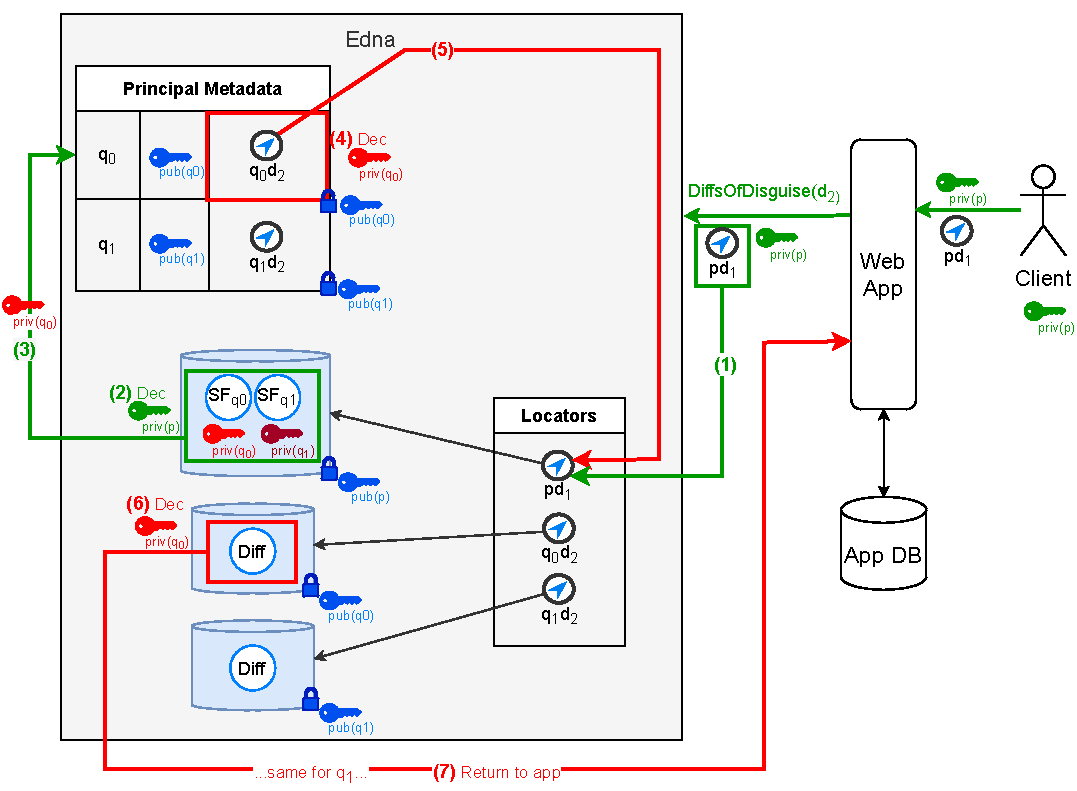
\includegraphics[width=0.5\textwidth]{figs/edna_reveal}
    \caption{\sys composes disguises by recursively disguising
             pseudoprincipal-owned records.}
    \label{f:recursive}
\end{figure}

%
We imagine that \sys-enabled applications will contain multiple
disguises, and that developers will invent and implement new disguises
over time.
%
For example, an application might start out with a disguise for account
deletion only, then add a data decay disguise, and finally add a more
fine-grained anonymization disguise that scrubs identifying keywords
from content in addition to decorrelating them.
%
Or a disguise may have a bug that requires an additional disguise
to remedy.
%
In all these cases, \sys must support disguises that potentially
operate over already-disguised data.
%

%
The application database changes for a disguise $d_2$ that applies
to data already disguised by earlier disguise $d_1$ are fairly
straightforward: $d_2$ modifies the data again, deletes it, or
decorrelates it to pseudoprincipals.
%
However, if \sys is to permit revealing $d_2$---\ie let a natural
principal $p$ restore the state after as it was $d_1$ but before
$d_2$---it must store encrypted records of $d_2$'s changes.
%
But now, a challenge arises: data decorrelated to pseudoprincipals
by $d_1$ is owned by those pseudoprincipals in the application
DB, rather than with a natural principal; indeed, the application
and \sys \emph{must} have forgotten the association with a natural
principal to be secure.
%
Thus, \sys lacks a public key to encrypt $d_2$'s changes for $p$.
%
Moreover, the application cannot convey the locators returned by
\sys to a client without knowing the natural principal.
%

%
To solve this challenge, \sys stores data for pseudoprincipals,
and establishes ways for a natural principal to prove a speaks-for
relationship with these pseudoprincipals.
%
For example, after the instructor anonymizes a class in WebSubmit, all
answers are associated with pseudoprincipals.
%
If the instructor later decides to scrub identifiers from answer contents
using another disguise, those disguise's will be associated with
pseudoprincipals.
%
%However, if a client speaking for the pseudoprincipals interactively applies the disguise (\eg a user
%deletes $p$'s account after anonymization), the deletion disguise's records can be associated with
%$p$, rather than the pseudoprincipals that own $p$'s data after anonymization.
%

\head{Storing Data for Pseudoprincipals.}
%
\sys must store data for pseudoprincipals in such a way that only a client
with natural principal $p$'s private key can access the records of $p$'s
pseudoprincipals.
%
%Encrypting records for pseudoprincipal $q$ with $p$'s public key does not
%always work, as \sys may not know which natural principal $p$ links to $q$.
%
Each time \sys creates a new pseudoprincipal $q$ for natural principal $p$,
it also generates a keypair for $q$.
%
Just like with natural principals, \sys stores $q$'s public key and uses it
to encrypt $q$'s records.
%
\sys then ``wraps'' $q$'s private key by encrypting it with $p$'s public key,
and forgets the plaintext private key.
%
As a result, access to $q$'s private key requires $p$'s private key, and, thus
access to future records in \sys encrypted for $q$ does as well.
%
\sys stores $q$'s wrapped private key at location \lcapa{pd} along with
$p$'s encrypted data.
%

%
Finally, this idea applies recursively: in the above example, $p$ itself may
be a pseudoprincipal $r$ and not a natural principal.
%
(This is why the application cannot \eg simply email $q$'s private key to
$p$ when it creates a pseudoprincipal $q$.)
%
In this case, \sys encrypts $q$'s private key with the public key of
pseudoprincipal $r$, granting any natural principal who can access
$r$'s private key access to $q$ and its data.
%

\head{Storing Pseudoprincipals' Locators.}
%
When a disguise $d_2$ generates records owned by a pseudoprincipal $q$, \sys
stores these encrypted records at some locator.
%
If the call to store the record indicates an interactive client speaking-for $p$,
\sys stores the ciphertexts at \lcapa{pd}, and everything is fine (\lcapa{pd} is sent back to the
client).
%
If \sys is not applying the disguise on behalf of a particular user, however, \sys stores encrypted records at some locator for $q$, \lcapa{qd}.
%
In this case, the application and \sys have nowhere to send \lcapa{qd} when the disguise completes, because $q$ is a
pseudoprincipal.
%
To retain the ability to efficiently access the records via \lcapa{qd}, \sys encrypts \lcapa{qd}
with the pseudoprincipal's public key and stores the resulting ciphertext in \sys's metadata for $q$
(which also includes $q$'s public key).
%
It is fine to encrypt the locator, since it will only be needed to reveal
the disguise---and at that point, $q$'s private key will be available,
as the principal who speaks-for $q$ can unwrap it.
%

\head{Pseudoprincipal Metadata.}
%
\fn{ForgetPrincipal} tells \sys to remove any metadata about a principal
$p$.
%
However, \sys must sometimes retain part of $q$'s metadata, as it may include
encrypted locators that \sys must keep to later efficiently find $q$'s
encrypted record bags.
%
Given that \sys cannot decrypt $q$'s locators, nor send them to a
client, \sys retains pseudoprincipal metadata if it contains encrypted locators
when the application calls \fn{ForgetPrincipal}.
%
However, \sys records that the pseudoprincipal is forgotten, so that \sys
knows to delete $q$'s metadata when future \fn{ForgetData} calls remove
the locators.
%

%
\sys removes a pseudoprincipal locator \lcapa{qd_2} when the application
decides that data from disguise $d_2$ is no longer needed (\eg because
the disguise has been revealed).
%
The application calls \fn{ForgetData($d_2$, \lcapa{pd_1})} with a
user-provided locator that must necessarily be from an earlier disguise
$d_1$ that decorrelated $q$ from natural principal $p$.
%
\lcapa{pd_1} allows \sys to access $q$'s private key, decrypt $q$'s locator
\lcapa{qd_2}, and drop the bag at \lcapa{qd_2}.
%
Once this is done, \sys removes \lcapa{qd_2}.
%

%
Because \sys may need to use \lcapa{pd_1} to access $q$'s encrypted private key,
\sys retains $q$'s encrypted private key at \lcapa{pd} even if a prior call to
\fn{ForgetData($d_1$, \lcapa{pd_1})} removed the rest of $d_1$'s data under
disguise at \lcapa{pd_1} (\ie encrypted diff or speaks-for records).
%
To obscure that the bag is empty except for $q$'s private key,
\sys puts a random-length dummy record into the bag; this hides that \sys
deleted previously-stored data.
%
%Once \sys has removed $q$'s metadata, then \sys removes all trace of
%\lcapa{pd} since the referenced bag is empty.
%

\head{Putting It Together.}
%
Figure~\ref{f:recursive} shows an example of how a client that provides
the private key natural principal $p$ and locator \lcapa{pd_1} accesses
\emph{both} $p$'s records for disguise $d_1$, the private
keys of all pseudoprincipals ${q_0, \dots, q_k}$ created during disguise
$d_1$, and all records encrypted for these pseudoprincipals during disguise
$d_2$.

%
In the first case, $p$ did not interactively apply $d_2$, and thus \sys does not have $p$'s private
key or locators.
\sys accesses $q_i$'s private key by decrypting (with $p$'s private key) the
bag at \lcapa{pd_1} that contains the wrapped private key.
Since $p$ did not invoke $d_2$, \sys stored a locator for $q_i$'s encrypted records
\lcapa{q_id_2} in $q\_i$'s metadata.
With $q_i$'s private key, \sys decrypts \lcapa{q_id_2} from $q_i$'s metadata,
and uses it to locate $q_i$'s encrypted records from $d_2$, decrypting the records
with $q_i$'s private key.
%

%
In the second case, $p$ interactively invoked $d_2$. \sys thus created a locator \lcapa{pd_2} for
$q_i$'s records and sent this to $p$; $q_i$ has no affiliated encrypted locators. To access $q_i$'s
records for disguise $d_2$, a client can simply provide \lcapa{pd_2} in addition to \lcapa{pd_1} and
$p$'s private key. \sys still first retrieves $q_i$'s private key with $p$'s private key and
\lcapa{pd_1}, and then uses \lcapa{pd_2} and $q_i$'s private key to directly locate $q_i$'s
encrypted records and decrypt them.
%

%%%%%%%%%%%%%%%%%%%%%%%%%%%%%%%%%%%%%%%%%%%%%%%%%%%%%%%%%%%%%%%%%%%%%%%%%%%%%%%%%%%%%%%%%%
%%%%%%%%%%%%%%%%%%%%%%%%%%%%%%%%%%%%%%%%%%%%%%%%%%%%%%%%%%%%%%%%%%%%%%%%%%%%%%%%%%%%%%%%%%
%%%%%%%%%%%%%%%%%%%%%%%%%%%%%%%%%%%%%%%%%%%%%%%%%%%%%%%%%%%%%%%%%%%%%%%%%%%%%%%%%%%%%%%%%%
%%%%%%%%%%%%%%%%%%%%%%%%%%%%%%%%%%%%%%%%%%%%%%%%%%%%%%%%%%%%%%%%%%%%%%%%%%%%%%%%%%%%%%%%%%
%%%%%%%%%%%%%%%%%%%%%%%%%%%%%%%%%%%%%%%%%%%%%%%%%%%%%%%%%%%%%%%%%%%%%%%%%%%%%%%%%%%%%%%%%%
%%%%%%%%%%%%%%%%%%%%%%%%%%%%%%%%%%%%%%%%%%%%%%%%%%%%%%%%%%%%%%%%%%%%%%%%%%%%%%%%%%%%%%%%%%
%%% OLD
\begin{comment}
%%%%%%%%%%%%%%%%%%%%%%%%%%%%%%%%%%%%%%%%%%%%%%%%%%%%%%%%%%%%%%%%%%%%%%%%%%%%%%%%%%%%%%%%%%
\section{Disguising and Revealing Semantics}
\label{sec:comp}
%%%%%%%%%%%%%%%%%%%%%%%%%%%%%%%%%%%%%%%%%%%%%%%%%%%%%%%%%%%%%%%%%%%%%%%%%%%%%%%%%%%%%%%%%%
This section describes the semantics of disguising provided by \sys.
In particular, we describe the end state of a data object given some history of disguise
applications and reveals.

\vspace{6pt}\noindent\textbf{\emph{Some Notation.}} We describe disguise histories as a list of
\app{d_i} and \rev{d_i} actions, where \app{d_i} corresponds to the application of disguise $d_i$, and
\rev{d_i} corresponds to the reveal of $d_i$'s diffs. Time moves to the right in the list.

For every data object $x$ in the system, \xstart describes its initial state, and
\xhist{[\app{d_1}, \dots]} describes its state after \sys has applied the history [\app{d_1},
$\dots$].


%%%%%%%%%%%%%%%%%%%%%%%%%%%%%%%%%%%%%%%%%%%%%%%%%%%%%%%%%%%%%%%%%%%%%%%%%%%%%%%%%%%%%%%%%%
\vspace{6pt}\noindent\textbf{\emph{Composing Multiple Disguise Applications.}}
Let $d_1$ and $d_2$ be two disguises, where $d_1$ is applied after $d_2$.
to produce disguise history [\app{d_1}, \app{d_2}].
%
Let $x$ be some application data object, where \xstart is its initial state, and
\xhist{[\app{d_1}, \app{d_2}]} is the final state after \sys applies $d_1$ and $d_2$.
%
If both $d_1$ and $d_2$ update $x$, what is \xhist{[\app{d_1}, \app{d_2}]}?
We consider two possible end states:
%
\begin{enumerate}
    \item[(\appcompone)] \xhist{[\app{d_1}, \app{d_2}]} reflects the application of
        \emph{both $d_1$ and $d_2$} to \xstart.

        In other words, if an \op{d_2}'s predicate \texttt{pred} matches \xstart, then \op{d_2} is
        applied to \xhist[\app{d_1}], even if \texttt{pred} does not match
        \xhist{[\app{d_1}]}.

    \op{d_2} updates are applied sequentially after $d_1$'s updates if the two modify the
        same object attribute.

\item[(\appcomptwo)] \xhist{[\app{d_1}, \app{d_2}]} reflects the application of $d_1$ to \xstart, followed
by the application of $d_2$ to \xhist{[\app{d_1}]}. When deciding whether to apply to $x$,
        \sys matches \op{d_2}'s predicate only against
\xhist{[\app{d_1}]}, and not against the original state \xstart.
\end{enumerate}

\noindent
For example, let \op{d_1} decorrelate all posts from authors predicated on \texttt{author =
Bea}, and let \op{d_2} remove all posts predicated on \texttt{author = Bea}.
%
\begin{enumerate}
\item[(\appcompone)] Both \op{d_1} and \op{d_2} update posts originally having author ``Bea'', resulting in the
removal of all posts originally with author Bea.

\item[(\appcomptwo)] Applying \op{d_1} results in all posts with author ``Bea'' having
pseudoprinicipal authors such as ``anonFox.'' \op{d_2} only knows the state of posts after
\op{d_1} occurs, and does not remove any posts because no post has author ``Bea''.
\end{enumerate}

The choice of whether \xhist{[\app{d_1}, \app{d_2}]} should result in \appcompone or \appcomptwo depends on the
specific application and is left to the developer to specify.

In certain scenarios, however, \sys can only achieve end state \appcomptwo. In order to achieve \appcompone,
$d_2$ must evalute predicates against \xstart, which requires knowing the value of \xstart.  To learn
\xstart, \sys must know how $d_1$ modified $x$ (\eg knowing that a post with author ``anonFox''
originally was a post with author ``Bea''); this information, however, is stored in in the diffs produced
by $d_1$.

\sys may not have access to these diffs when applying $d_2$: a client who invokes $d_2$ while authenticated as
principal $q \neq p$, and who does not provide the relevant capabilities%y pairs \pcapa{pd_1},
cannot access $p$'s diffs for $d_1$.

In this case, $d_2$ can only match against \xhist{[\app{d_1}]} and achieve end state \appcomptwo.
This is shown in Table~\ref{tab:composeapp}.

\begin{table}[h]
\centering
\begin{tabular}{ c | c c }
    & \multicolumn{2}{c}{\textbf{Access $d_1$'s diffs while \app{d_2}?}}\\
    & \textbf{Yes} & \textbf{No} \\
\hline
    \xhist{[\app{d_1},\app{d_2}]}& \appcompone or \appcomptwo & \appcomptwo
\end{tabular}
\vspace{6pt}

\caption{Possibilities for \xhist{[\app{d_1},\app{d_2}]} depending on whether \sys has access to diffs from $d_1$ regarding $x$.}
\label{tab:composeapp}
\end{table}

%%%%%%%%%%%%%%%%%%%%%%%%%%%%%%%%%%%%%%%%%%%%%%%%%%%%%%%%%%%%%%%%%%%%%%%%%%%%%%%%%%%%%%%%%%
\vspace{6pt}\noindent\textbf{\emph{Semantics of Disguise Reversals.}}
We now consider composition of disguises in the presence of disguise reversals.

\begin{table}[h]
\centering
\begin{tabular}{ c | c c }
    & \multicolumn{2}{c}{\textbf{Access to $d_i$'s diffs while \app{d_i}?}}\\
    & \textbf{Yes} & \textbf{No} \\
\hline
    \xhist{[\app{d_i},\rev{d_i}]} & \xstart & \xhist{[\app{d_i}]}
\end{tabular}
\vspace{6pt}

\caption{Possibilities for \xhist{[\app{d_i},\rev{d_i}]} depending on whether \sys has
    access to diffs from $d_i$ regarding $x$.}
\label{tab:composeapprev}
\end{table}

We first consider \textbf{\xhist{[\app{d_i},\rev{d_i}]}}; Table~\ref{tab:composeapprev}
illustrates how this state depends the authorization a client invoking \rev{d_i} provides to
\sys to access $d_i$'s diffs for $x$.
As expected, the updates applied by $d_i$ to $x$ cannot be revealed when the relevant diffs are
inaccessible.

\begin{table}[h]
\centering
\begin{tabular}{ c | c c }
    \textbf{$d_1$ and $d_2$'s Updates} & \multicolumn{2}{c}{\textbf{Access
        to $d_1$'s diffs while \rev{d_1}?}}\\
    & \textbf{Yes} & \textbf{No} \\
    \hline
    \textbf{Independent} & \xhist{[\app{d_2}]} & \xhist{[\app{d_1},\app{d_2}]}\\
    \textbf{Conflict} & \xhist{[\app{d_1},\app{d_2}]} & \xhist{[\app{d_1},\app{d_2}]}
\end{tabular}
\vspace{6pt}
    \caption{\xhist{[\app{d_1},\app{d_2},\rev{d_1}]} depending on whether \sys has
    access to $d_1$'s diffs when revealing $d_1$, and whether updates from $d_1$ and
    $d_2$ to $x$ modify the same data.}
\label{tab:composeapprev1}
\end{table}

We next consider \textbf{\xhist{[\app{d_1},\app{d_2},\rev{d_1}]}}: the end state of $x$ when a disguise
$d_1$ is revealed after a subsequent disguise $d_2$ has been applied.
Table~\ref{tab:composeapprev1} illustrates how the result
depends on \sys's access to $d_1$ diffs, and whether $d_1$ and $d_2$ performed
conflicting modifications to $x$'s attributes.

When the client invoking \rev{d_1} provides no authorization to access to $d_1$'s diffs, then the
updates applied by $d_1$ to $x$ cannot be revealed.  However, even if the client
grants access to $d_1$'s diffs, \sys will fail to reveal $d_1$'s updates to $x$ if $d_2$ and $d_1$
both modify $x$ in a conflicting manner: $\rev{d_1}$ must not restore data that was also disguised by
$d_2$, and until $d_2$ is revealed, invocations of \rev{d_1} will not reveal \xstart.

\subsection{Composition Implementation Techniques}
\sys's algorithm for disguising and disguise reversal in most scenarios is straightforward.

To apply disguise $d_i$, \sys applies each \op{d_i} to all
data objects satisfying \op{d_i}'s predicate, while also taking into account the information in
accessible diffs(to \eg predicate against undisguised versions of objects). Each \op{d_i} produces
one or more diffs, which \sys stores either globally or encrypted by a data capability at
\lcapa{pi_i}.

To reveal disguise $d_i$, \sys reveals the undisguised version of data stored in
accessible diffs corresponding to $d_i$ by updating the relevant objects $x$ in the database.

However, \sys must be careful of two potential problems:
(1) \sys cannot accidentally reveal data that must be disguised; and (2) \sys cannot let global
diffs recording updates to data $x$ leak information if $x$ is subsequently (privately) disguised.

%%%%%%%%%%%%%%%%%%%%%%%%%%%%%%%%%%%%%%%%%%%%%%%%%%%%%%%%%%%%%%%%%%%%%%%%%%%%%%%%%%%%%%%%%%
\vspace{6pt}\noindent\textbf{\emph{Preventing Accidental Data Revelation.}}
\sys records the disguised state of data $x$ in each \tdiff{pd} recording a update performed by $d_i$
to $x$. If the state of $x$ does not match the disguised state in $d_i$'s diff for $x$, then \sys
knows the diff records a stale and overwritten update to $x$, and refuses to reveal the undisguised state of $x$
stored in the diff.

%%%%%%%%%%%%%%%%%%%%%%%%%%%%%%%%%%%%%%%%%%%%%%%%%%%%%%%%%%%%%%%%%%%%%%%%%%%%%%%%%%%%%%%%%%
\vspace{6pt}\noindent\textbf{\emph{Preventing Global Diff Information Leakage.}}
%The ONLY REASON we need to update diffs is if they're global!!! If they're private, we can use the
%retroactive application method... (optimization to update our "own" diffs though)
%
A disguise may optionally store diffs in global storage, accessible to \sys without any client
authorization.
Such a global disguise provides no privacy guarantees against an adversary who compromises
the application server, but does transform the application database so external users see disguised
data.

If $d_1$ is a global disguise and $d_2$ a normal, privacy-preserving disguise,
\op{d_2} may update a data object $x$ previously updated by \op{d_1}.

\op{d_1} produces a global diff \tdiff{pd_1}; \op{d_2} produces a normal,
encrypted and secured diff \tdiff{pd_2}.

If \sys simply performs \op{d_2}'s update to $x$, an adversary can still read undisguised data
from the \tdiff{pd_1} diff because the diff is global and records a now-stale state of $x$!
%
To prevent global diffs like \tdiff{pd_1} from leaking data that should be disguised, \sys
updates the data in \tdiff{pd_1} with \op{d_2}'s update. An update to a diff such as
\tdiff{pd_1} itself generates a (private) diff \tdiff{pd_2}, just as updating a data
object generates a diff.

Revealing $d_2$ uses \tdiff{pd_2} to reveal the modification to \tdiff{pd_1}.
If $d_1$ has already been revealed, and the database state of $x$ updated to reflect the
contents of \tdiff{pd_1} (which were updated by the application of $d_2$), then \sys
simply uses \tdiff{pd_2} to reveal the current state of $x$ in the database.

If a future $d_3$ has further updated \tdiff{pd_1} in a way that conflicts with $d_2$'s update, then
upon reversal of $d_2$, \sys will notice that \tdiff{pd_2} records an overwritten update to
\tdiff{pd_1}, and will not revert the state of \tdiff{pd_1} until the future disguise $d_3$ has been
revealed .

\lyt{Note that removal is just an interesting case of this, in which \tdiff{pd_1} is removed, by a
diff \tdiff{pd_2} stored in \lcapa{pd_2} that saves the removal of \tdiff{pd_1} for reversal.}

%\vspace{6pt}\noindent\textbf{\emph{diff Modification for Object Identification.}}
%diffs need to refer to the correct objects even if objects have been modified by future disguises.
%Prior diffs should be revised by future disguises so that they apply correctly to the disguised
%data.
%This allows an earlier disguise to be revealed correctly.
%An easy way to avoid needing to do this is to have all objects in the DB have unique, permanent
%identifiers.
\end{comment}
